\chapter[Metodologia]{Metodologia}

\section{Metodologia para pesquisa e construção do produto}

\subsection{Estrutura}
Modelagem 3D do dispositivo: será construído um modelo 3D da estrutura, seguindo as dimensões especificadas pela \cite[p.~97]{nbr9050} e as dimensões do IMETRO, utilizando para isto o software Catia V5 3D.

\subsection{Power Train}

\subsubsection{Motor}
O motor é uma máquina que tem a capacidade de transformar energia elétrica em energia mecânica \cite{projeto_cadeira_rodas_inteligente}, existem dois tipos de motores, motor de corrente alternada (ca) e os de corrente contínua (cc). Será avaliado qual o tipo se encaixa melhor aos requisitos do projeto.

\subsubsection{Bateria}
Baterias são dispositivos que transformam energia química em elétrica e vice-versa. Por ser um processo reversível, as baterias podem ser carregadas e descarregadas várias vezes. Hoje no mercado existem vários tipos de baterias, com diferentes condições nominais, serão levantados os requisitos necessários e qual tipo de bateria se adéqua melhor ao projeto.

\subsection{Controle}
Levantamento das possíveis interfaces humano- computador visando a melhor ergonomia e conforto do usuario. Estudo das possiveis tecnologias para o controle do motor e linguagem computacional.

\section{Metodologia de organização e monitoramento}

Para a execução do projeto o grupo organizou com base nas metodologias ágeis “Extreme Programming” (XP) e Scrum, comuns a engenharia de software, porém, estas metodologias foram adaptadas conforme a necessidade e o contexto do projeto que este documento descreve. Um exemplo destas adaptações é a ausência de um “Product Owner”, para esta representação todo o grupo a exercerá através de reuniões para tomadas de decisão.

O Scrum e o XP são metodologias ágeis que nos baseamos para o planejamento do processo produtivo. No inicio do projeto foi definido o escopo, product backlog, de uma forma mais macro, resultando assim na nossa EAP, que pode ser observada na figura \ref{fig:eap}.

\begin{figure}[!htb]
\centering
  \includegraphics[keepaspectratio=true,scale=0.5]{figuras/metodologia/EAP}
\caption{EAP}
\label{fig:eap}
\end{figure}

O projeto foi dividido em Sprints, técnica do Scrum baseada em intervalos fixos de tempo para a entrega de uma parte do produto final (Builds), que por votação interna teve sua duração limitada a uma semana. Foi definido também que a cada inicio de Sprint será realizada Planning, reunião dedicada ao planejamento de toda a Sprint. Em seu decorrer será realizado dailies, um feedback diário de cada membro, ou cada pairing do que foi realizado naquele dia, se existe alguma dificuldade e o que será feito no próximo dia. No final da Sprint será realizado uma retrospectiva onde são levantados pontos positivos e pontos a serem melhorados.

A presença dos integrantes do grupo nos horários de aula serão obrigatórios e controlados através de lista de presença de controle interno, pois devido as Sprints de duração de uma semana o Planning e retrospectiva serão realizados nas aula de sexta-feira, e quarta feira será realizado um ponto de controle interno que pode servir tanto para a realização de super-pairings, quanto para tomadas de decisões importantes para o andamento do projeto.
Os prazos e datas nos quais foram baseados as datas de entrega, builds, releases, foram definidos para se adequar ao tempo da disciplina e às datas estipuladas pelo plano de ensino da disciplina. Com isso foi feito o planejamento de Sprints que pode ser encontrado na figura \ref{fig:cronograma}

\begin{figure}[!htb]
\centering
  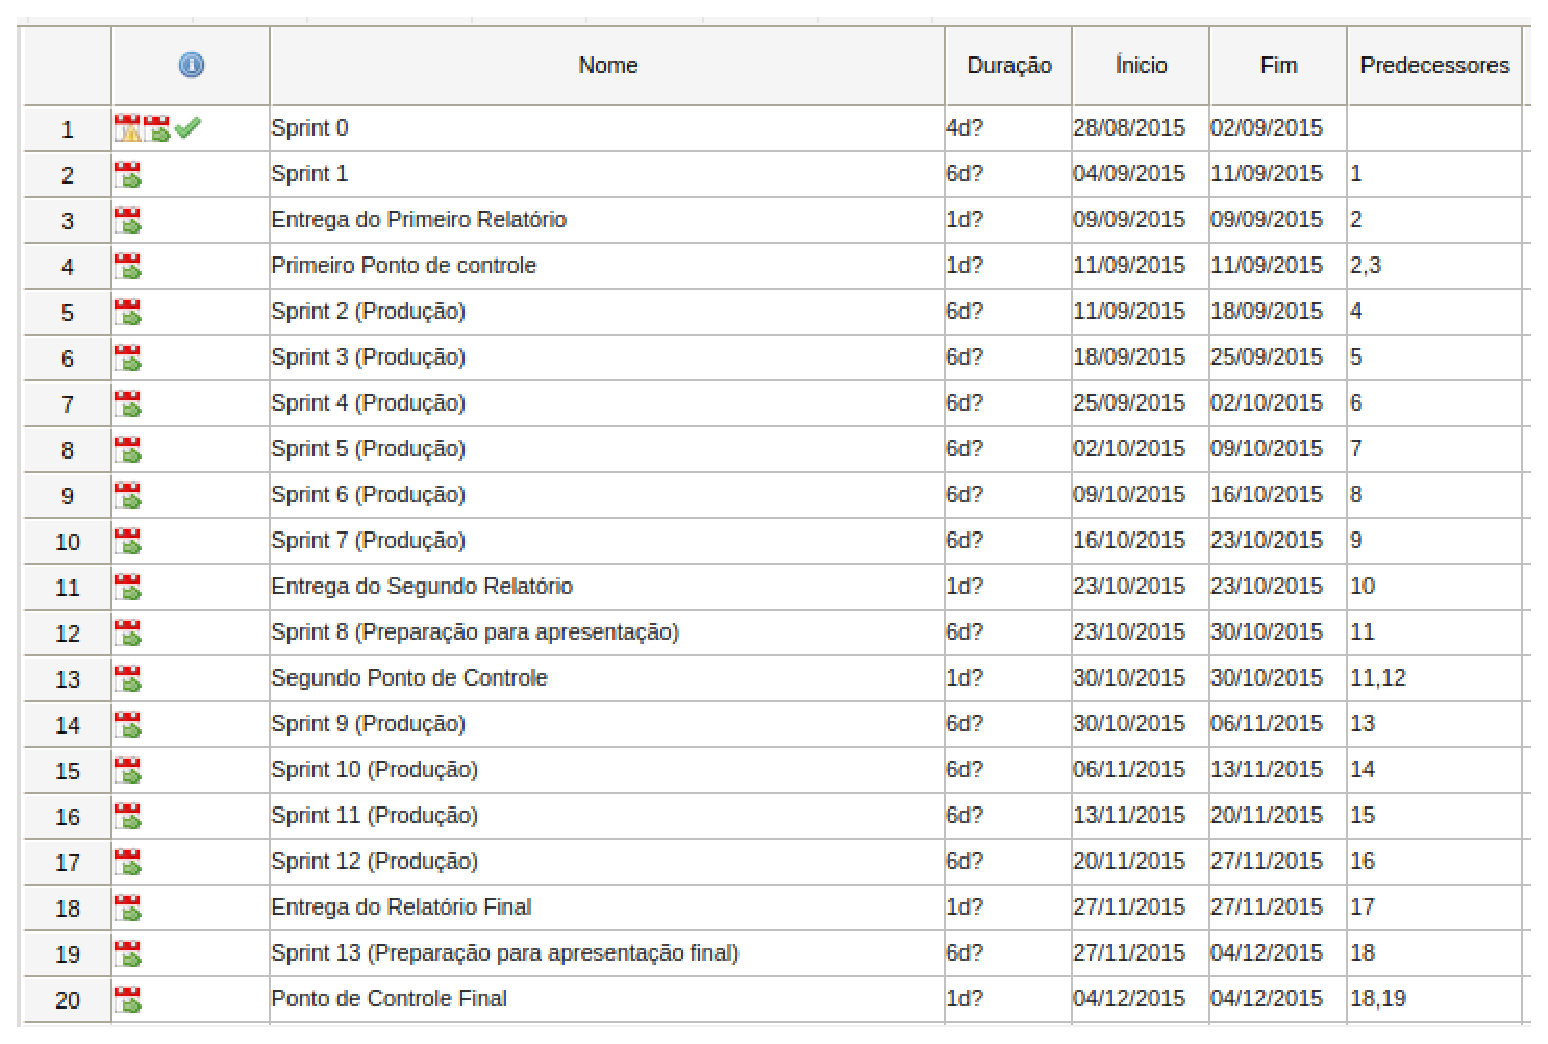
\includegraphics[keepaspectratio=true,scale=0.5]{figuras/metodologia/cronograma}
\caption{EAP}
\label{fig:cronograma}
\end{figure}

Para o acompanhamento do projeto serão utilizadas ferramentas que facilitam os métodos citados anteriormente. Para auxiliar na comunicação será utilizada a ferramenta Slack, para o compartilhamento de Artefatos, pesquisas e documentos será utilizada a ferramenta Google Drive, para reuniões à distancia será utilizada a ferramenta Google Hangouts, para o desenvolvimento  e versionamento dos softwares provenientes será utilizado o GitHub.

Com isso podemos concluir que nossas fases são divididas em Sprints, e as atividades são definidas no planejamento inicial de cada Sprint, bem como os responsáveis. As entradas são as atividades planejadas e as saídas são os relatórios e o produto incrementado. Os prazos limitadores serão o final de cada Sprint, e o critério de conclusão o aceite interno da equipe juntamente com o feedback dos professores orientadores
